\documentclass[11pt]{article}
\usepackage{classTools}

\begin{document}

\psHeader{1}{Wed 2024-09-18 (11:59pm)}

Please review the Syllabus for information on the collaboration policy, grading scale, revisions, and late days.

Unfortunately, we made a few mistakes in our previous iteration of trying to use GitHub Classroom--this time, we have (hopefully) figured out those wrinkles and have a \href{https://classroom.github.com/a/hCzdB8ze}{new GitHub Classroom assignment} for you all to accept. If you were initially using a fork of the public repo, we recommend using Classroom, since we'll be able to post things like practice materials, section notes, and problem set solutions which we usually don't want to display on the public repository. This time you should be able to easily access updates by viewing your repo on the website, clicking on the pull request and accepting it (more details on Ed to come).


\begin{enumerate}
    \item (Asymptotic Notation) 
    \begin{enumerate}
    \item (practice using asymptotic notation)
        Fill in the table below with ``T'' (for True) or ``F'' (for False) to indicate the relationship between $f$ and $g$. For example, if $f$ is $\Omega(g)$, the first cell of the row should be ``T.''   No justification necessary.  Notice that some of the functions are the same as in Problem Set 0.\\
        \begin{table}[h!]
        \centering
        \bgroup
        \def\arraystretch{1.3}
        \begin{tabular}{||c | c || c | c | c | c | c ||}
         \hline
         $f$ & $g$ & $\Omega$ & $\omega$ & $\Theta$ \\
         \hline\hline
         $3\log ^3 n$ & $n^2+1$ & F & F & F \\ \hline
         $4n^3$ & $\left| \{S \subseteq [n] : |S|\leq 3\}\right|$ & T & F  & T \\ \hline
         $n!$ & $5^n$ & F & F & F \\ \hline
         $3^n$ & $\left(2+(-1)^n\right)^n$ & T & F & F\\ \hline
        \end{tabular}
        \egroup
        \end{table}
        Recall that, throughout CS1200, all logarithms are base 2 unless otherwise specified. 
        
    \item  (runtimes: $T^=$ vs. $T$)  
    Let $g : \R^{\geq 0}\rightarrow \R^{\geq 0}$ be a nondecreasing function, i.e. if $x\geq y$, then $g(x)\geq g(y)$. (For example $g(n)=n^2$, $g(n)=n\log n$, or $g(n)=2^n$.) Let $T^{=} : \N\rightarrow \N$ and $T : \R^{\geq 0}\rightarrow \N$ be the runtimes of an algorithm $A$, as defined in Lecture 2. 
    \begin{enumerate}   
    \item Prove that $T^{=}=O(g)$ iff $T=O(g)$. Thus the distinction between $T$ and $T^{=}$ does not matter when we are interested in natural runtime bounds, which are nondecreasing. 
    \\
    \\ To prove both ways, we need to prove the individual sides of the claim first.
    \\\\ (1) If $T = O(g)$, then $T^{=}=O(g)$
    \\ We know that by the definition of the big-O relationship, there exists a $c : c > 0$ such that for all large enough $n \geq n_0$:
    \begin{equation*}
        T(n) \leq c \cdot g(n)
    \end{equation*}
    Because we know that $T(n) = max(T^{=}(n)$ for all $n \geq n_0$, we can then say:
    \begin{equation*}
        max(T^{=}(n)) = T(n) \leq c \cdot g(n)
        \Rightarrow T^{=} \leq c \cdot g(n)
    \end{equation*}
    So, $T^{=}=O(g)$
    \\\\
    (2) If $T^{=}=O(g)$, then $T=O(g)$
    \\\\
    We know that by the definition of the big-O relationship, there exists a $c : c > 0$ such that for all large enough $n \geq n_0$:
    \begin{equation*}
        T^{=} \leq c \cdot g(n)
    \end{equation*}
    By definition, $T(n) = max_{0\leq j \leq n}T^{=}(j)$ for any given n. So, to prove that $T(n) = O(g)$, we can show that for all $i \in [0, n]$, $ T^{=} \leq c \cdot g(n)$. Then, by definition that T(n) is just the max of $T^{=}(n)$, we can prove that $T(n) \leq c \cdot g(n)$.
    \\\\ There are two cases to check:
    \\\\ \textbf{Case 1: $i \in [n_0, n]$}. 
    \\ Since g is non-decreasing, that means that $g(i) < g(n)$. So, we can say that:
    \begin{equation*}
         T^{=}(i) \leq c \cdot g(i) \leq c \cdot g(n)
    \end{equation*}
    \\ \textbf{Case 2: $i \in [0, n_0)$}. 
    \\ In the same case as above, we know that g is non-decreasing. So, $g(n_0) < g(n_0 + 1)$. So, we can say that:
    \begin{equation*}
         T^{=}(i) \leq c \cdot g(i) \leq c \cdot g(n_0)
    \end{equation*}
    So, it is true that if $T = O(g)$, then $T^{=}=O(g)$
    \\ 
    \item  Let's consider the 4th case from the table, where $T^{=}(n) = (2 + (-1)^n)^n$ and $g(n) = 3^n$. Because $(-1)^n$ oscillates depending on the value of n, we know that for even n, $T^{=}(n) = 3^n$ and for odd n, $T^{=}(n) = 1^n = 1$
    \\\\ So, the value of $T^{=}(n)$ oscillates between $3^n$ and 1. In relation to $g(n)$, $T^{=}(n) \geq c \cdot g(n)$ only when c is non-constant and $c \leq 3^{-n}$. Because here, c is non-constant, we can say that $T^{=}(n) \neq \Omega(g)$.
    \\\\ But, even keeping $c = \frac{1}{3}$, we know that $T(n) \geq c \cdot g(n)$ for all cases. So, it is true that $T(n) = \Omega(g)$.
    \\\\ Hence we prove that the case that $T=\Omega(g) \Rightarrow T^{=}=\Omega(g)$ fails. 
    \end{enumerate}

 
    \end{enumerate}
    
    \newpage
    \item (Understanding computational problems and mathematical notation)\\\\
    Recall the definition of a {\em computational problem} from Lecture Notes 1.  \label{prob:BC}

 
    Consider the following computational problem $\Pi=(\Inputs,\Outputs,f)$: 
    \begin{itemize}                                
    \item $\Inputs = \N\times\N^{\geq 2}\times \N$, where $\N^{\geq 2} = \{2,3,4,\ldots\}$.  
    \item $\Outputs = \{(c_0,c_1,\ldots,c_{k-1}) : k,c_0,\ldots,c_{k-1}\in \N\}$
    \item $f(n,b,k) = \{ (c_0,c_1,\ldots,c_{k-1}) : n=c_0+c_1b+c_2b^2+\cdots+c_{k-1}b^{k-1}, \forall i\ 0\leq c_i< b\}.$ 
    \end{itemize}
Here is an algorithm $\BC$ to solve $\Pi$: 
    
\begin{algorithm}[H]
    \BC{$n,b,k$}\\
    {
    \ForEach{$i=0,\ldots,k-1$}{
    $c_i = n \bmod b$\;
    $n = (n-c_i)/b$\;
    }
    \lIf{$n==0$}{\Return{$(c_0,c_1,\ldots,c_{k-1})$}}
    \lElse{\Return{$\bot$}}}
\end{algorithm}


\begin{enumerate}
\item The output is {5, 3, 0, 0} because 35 can be written as:
\begin{equation*}
    35 = 5\cdot10^0 + 3\cdot10^1 + 0\cdot10^2 + 0\cdot10^3
\end{equation*}
\item Here, we give 3 numbers as input. We have the the number $n$, the base $b$, and number of digits $k$. The number $n$ is what we are trying to break down. We want to rewrite $n$ as a combination of base $b$, using $k$ terms. If we fail to rewrite it in terms of b, we return that we cannot.
\item Yes, there are $x \in \Inputs$ such that $f(x)=\emptyset$. One example is the Input $b = 10$, $k = 1$, $n = 35$. In this case, there is no single digit representation of 35 that we can make using just one base of 10. So, the function should return fail.
\item For all $n < b^k$, which is what we need to not fail our condition and return null, the $|f(x)|$ is 1. That is because there is simply only one way to represent an n with the base b. However, in the case that $n \geq b^k$, $|f(x) = 0|$ because the algorithm returns $\perp$.
\item  No, not every algorithm that solves $\Pi$ also solves $\Pi$'. An example would be when $n < b^k$. In both cases, algorithm A will return $\perp$ because $\Pi$ should return nothing in this case. However, $\Pi$' has a valid output in the form $(0, 1, ...., k-1)$, which A fails to return.


\end{enumerate}
\newpage

\item (Radix Sort) In the Sender--Receiver Exercise associated with lecture 3, you studied the sorting algorithm \SingletonBucketSort, generalized to arrays of key--value pairs, and proved that it has running time $O(n+U)$ when the keys are drawn from a universe of size $U$. In this problem you'll study {\em \RadixSort}, which improves the dependence on the universe size $U$ from linear to logarithmic.  Specifically, \RadixSort\ can achieve runtime $O(n+n\cdot (\log U)/(\log n))$, so it achieves runtime $O(n)$ whenever $U = n^{O(1)}$.  

\RadixSort\ is constructed by using \SingletonBucketSort\ as a subroutine several times, but on a smaller universe size $b$.  Specifically, it turns each key from $[U]$ into an array of $k$ subkeys from $[b]$ using the algorithm \BC\ from Problem~\ref{prob:BC} above as a subroutine, and then iteratively sorts on each of the $k$ subkeys,
Crucially, \RadixSort\ uses the fact that \SingletonBucketSort\ can be implemented in a way that is {\em stable} in the sense that it preserves the order in the input array when the same key appears multiple times.  (See the ``Food for Thought'' section in the SRE notes.)  Here is pseudocode for \RadixSort:


\begin{algorithm}[H]
\RadixSort{$U,b,A$}\\
\Input{A universe size $U\in \N$, a base $b\in \N$ with $b\geq 2$, and an array $A=((K_0,V_0),\ldots,(K_{n-1},V_{n-1}))$, where each $K_i\in [U]$}
\Output{A valid sorting of $A$}
%$b=\min\{n,U\}$\;
$k=\lceil \log_b U\rceil$\;
%$k=\lceil (\log U)/(\log b)\rceil$\;
\ForEach{$i=0,\ldots,n-1$}{
    $V_i' = \BC(K_i,b,k)$ \tcc*{$V_i'$ is an array of length $k$}}
\ForEach{$j=0,\ldots,k-1$}{
    \ForEach{$i=0,\ldots,n-1$}{
    $K'_i = V'_i[j]$
    }
    $((K_0',(V_0,V'_0)),\ldots,(K_{n-1}',(V_{n-1},V'_{n-1}))) = \SingletonBucketSort(b,((K'_0,(V_0,V_0')),\ldots,(K'_{n-1},(V_{n-1},V'_{n-1})))$\;
}
\ForEach{$i=0,\ldots,n-1$}{
    $K_i = V'_i[0]+V'_i[1]\cdot b + V'_i[2]\cdot b^2+\cdots+V'_i[k-1]\cdot b^{k-1}$}
\Return{$((K_0,V_0),\ldots,(K_{n-1},V_{n-1}))$}
\caption{Radix Sort}
\end{algorithm}

(You can also read a description of Radix Sort in CLRS Section 8.3 for the case of sorting arrays of keys (without attached items) when $U$ and $b$ are powers of 2, albeit using different notation than us.)

        \begin{enumerate}
        
            \item (proving correctness of algorithms) Prove the correctness of \RadixSort\ (i.e. that it correctly solves the SortingOnFiniteUniverse problem defined in SRE 1). 
            
            Hint: You will need to use the stability of \SingletonBucketSort in your argument. If it were replaced with an instable implementation (or any other unstable sorting algorithm, such as \ExhaustiveSearchSort\ with an unfortunate ordering on permutations), then the resulting algorithm would not be a correct sorting algorithm.   For intuition, you may want to think about what happens when you sort a spreadsheet by one column at a time. 
            \\
            \\ First of all, let's breakdown what the radix sort does in simpler terms. Basically, we are breaking down each key into smaller terms based on base b, and then comparing the values we multiply with our base terms to see which number is larger. We are using the singletonbucketsort on each of the subparts of the keys, and using the non-essential digits (right-most) before the left-digits.
            \\ Now, let's use induction to prove this works. 
            \\\\
            \textbf{Base Case:} When keys have only one subkey, or $k = 1$, the $\SingletonBucketSort $is only sorting through 1 subkey, so the sorting has to be correct.
            \\\\
            \textbf{Inductive Hypothesis:} Assume that for $k = m$ keys, the algorithm sorts the array correctly. 
            \\\\
            \textbf{Inductive Step:} For $k = m + 1$ keys, the algorithm sorts the array correctly. 
            \\\\
            \textbf{Inductive Proof:} 
            \\ First of all, the keys have $m + 1$ subkeys. To begin, the $\SingletonBucketSort$ will sort through the least significant digit first.
            \\ Then, because of the stability with $\SingletonBucketSort$, we know that as we sort the next subkeys, the order of the subkeys with the same value will not be disturbed, and the way they were sorted for previous subkeys will be preserved. 
            \\ So, sorting the $m$ subkeys, we will have a well sorted array as per the inductive hypothesis.
            \\ Now, we can invoke the stability of the $\SingletonBucketSort$ again to say that as we sort based on the $m+1$ subkey, we will not only get a correct sorting, but for all keys that will have the same value and are previously sorted, the order will be preserved. 
            \\
            
            \item (analyzing runtime) Show that \RadixSort\ has runtime $O((n+b)\cdot \lceil \log_b U\rceil)$.  Set $b=\min\{n,U\}$ to obtain our desired runtime of $O(n+n\cdot (\log U)/(\log n))$.  (This runtime analysis is outlined in CLRS, but you'd need to adapt it to our notation and slightly more general setting.) 
            \\\\
            Let's break this down into 3 different components of runtime:
            \\\\ \textbf{(1)} To convert the keys into subkeys: O(k).
            \\ Because there are n total keys, it means runtime would be O(nk). However, since $k = \lceil \log_b(U) \rceil$. we know that our runtime then is: $O(n \cdot \lceil \log_b(U) \rceil$.
            \\\\ \textbf{(2)} To sort the k subkeys with bucketsort: We have to go through $b$ buckets to first place the $n$ keys and then collect the $n$ keys. SO, the total is $O(n + n + b)$, but we also have to do so for all the $k$ subkeys. Then, the total goes to: $O(k(n + n + b))$.
            \\\\ \textbf{(3)} We have $O(n)$ to account for basic operations
            \\\\ Combining all terms, we get:
            \begin{equation*}
                O(n) + O(k(n + n + b)) + O(n\cdot \lceil \log_b U\rceil)
            \end{equation*}
            \begin{equation*}
                = O(n\cdot\lceil \log_b U\rceil) + O(\lceil \log_b U\rceil \cdot 2n + b) + O(n)
            \end{equation*}
            \begin{equation*}
                = O(n + b \cdot \lceil \log_b U\rceil)
            \end{equation*}
            
            \item (implementing algorithms)
            Implement \RadixSort\ using the implementations of \SingletonBucketSort\ and \BC\ that we provide you in the GitHub repository. 
  
            \item (experimentally evaluating algorithms) \label{part:graphs}
            In $\texttt{ps1\_experiments.py}$, we've provided code for running experiments to evaluate the runtime of sorting algorithms on random arrays (with $b=\min\{n,U\}$ in the case of \RadixSort) and for graphing the results. Run this code and attach the resulting graph (you should see that each sorting algorithm dominates in some region of the graph -- if you want better results you can try increasing the number of trials in the experiments file).
                
            \textit{Note: Your implementation of RadixSort, as well as any code you write for experimentation and graphing need not be submitted. Depending on your implementation, running the experiments could take anywhere from 15 minutes to a couple of hours, so don't leave them to the last minute!}   

            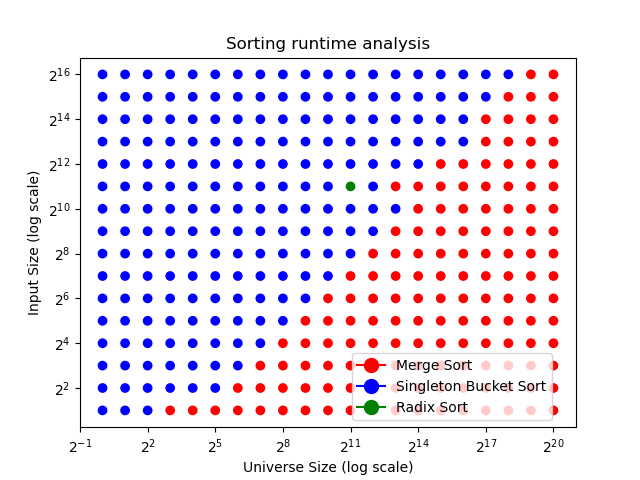
\includegraphics{Figure_1.png}
            
            \item Do the shapes of the transition curves found in Part~\ref{part:graphs} match what we'd expect from the asymptotic runtime formulas we have for the algorithms?  Explain.
            For a most thorough answer, try setting the asymptotic runtimes of \SingletonBucketSort\ and \RadixSort\ to be equal to each other (ignoring the hidden constant in $O(\cdot)$) and see what $\log U$ vs. $\log n$ relationship follows, and similarly for comparing \RadixSort\ and \MergeSort.
            \\ Every time I run, I get a different analysis, despite getting my code checked! It may be a computer issue, but I understand what I am supposed to be getting instead:
            \\\\ There should be a diagonal boundary between $\SingletonBucketSort$ and $\MergeSort$, with $\SingletonBucketSort$ being faster when input sizes get larger. That makes sense because the runtime of $\MergeSort$ is $O(n\cdot logn)$ versus for $\SingletonBucketSort$ it is $O(n + U)$. So, as n gets larger, the runtime for $\MergeSort$ should become worse because we are multiplying n by $logn$, instead of adding n and U like in $\SingletonBucketSort$.
            \\\\ Then, regarding the relationship between the $\MergeSort$ and the $\RadixSort$, the $\RadixSort$ should be better as the U and n become larger, but it still stays under the diagonal and is worse than $\SingletonBucketSort$. The reason why the $\MergeSort$ is slower than the $\RadixSort$ as n and U increase is because both the n and U increase together, and U is manageable enough that $logU$ is small enough that $\MergeSort$ is slower and $logn$ increases faster in contrast.
          
        \end{enumerate}

\item (Reflection Question)  There are a number of resources to support your learning in CS1200, such as Lecture, Ed, Office Hours, Section, Detailed Lecture Notes (posted after class), Recommended Readings, Collaboration with Classmates, the Patel Fellow, the Academic Resource Center (ARC), Sender-Receiver Exercises.  Which of these (or any others that come to mind) have you found most helpful so far and why?  Are there ones that you should take more advantage of going forward?  Do you have suggestions for how the course can make these more helpful to you?

\textit{Note: As with the previous pset, you may include your answer in your PDF submission, but the answer should ultimately go into a separate Gradescope submission form.}

\item Once you're done with this problem set, please fill out \href{https://forms.gle/Skby2L5TszNpSYDB6}{this survey} so that we can gather students' thoughts on the problem set, and the class in general. It's not required, but we really appreciate all responses!
\end{enumerate}

\end{document}